\documentclass[listings]{labreport}
\departmentsubject{Кафедра вычислительной техники}{Программирование интернет-приложений}
\titleparts{Лабораторная работа №2}{Вариант 78638}
\students{Калугина Марина, Каюков Иван}

\begin{document}

\maketitlepage

\section*{Цель работы}

Разработать веб-приложение на базе сервлетов и JSP, определяющее попадание точки на координатной плоскости в заданную область.

\begin{figure}[ht]
  \centering
  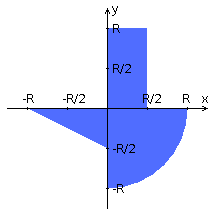
\includegraphics[width=6cm]{graph.png}
  \caption{Заданная область}
\end{figure}

Приложение должно быть реализовано в соответствии с шаблоном MVC и состоять из следующих элементов:

\begin{enumerate}
\item \textbf{ControllerServlet}, определяющий тип запроса, и, в зависимости
от того, содержит ли запрос информацию о координатах точки и радиусе, 
делегирующий его обработку одному из перечисленных ниже компонентов. 
Все запросы внутри приложения должны передаваться этому сервлету 
(по методу GET или POST в зависимости от варианта задания), 
остальные сервлеты с веб-страниц напрямую вызываться не должны.
\item \textbf{AreaCheckServlet}, осуществляющий проверку попадания 
точки в область на координатной плоскости и формирующий HTML-страницу 
с результатами проверки. Должен обрабатывать все запросы, содержащие 
сведения о координатах точки и радиусе области.
\item \textbf{Страница JSP}, формирующая HTML-страницу с веб-формой. 
Должна обрабатывать все запросы, не содержащие сведений о координатах 
точки и радиусе области.
\end{enumerate}

\section*{Исходный код}

Исходный код доступен по адресу \texttt{https://github.com/band-of-four/pipchansky}.

\section*{Вывод}

В данной лабораторной работе мы научились разрабатывать простые веб-приложения на базе сервлетов и JSP.

\end{document}
